\documentclass[fleqn,useAMS,usenatbib]{mnras}
%=====================================================================
% CUSTOM: PACKAGES, MACROS & SETTINGS
%=====================================================================
% packages for figures
\usepackage{graphicx,todonotes}

% packages for symbols
\usepackage{latexsym,amssymb}

% AMS-LaTeX package for e.g. subequations
\usepackage{amsmath,morefloats}
\usepackage{natbib,graphicx,amsmath,subfigure,color,xcolor,hyperref}
\usepackage{verbatim}

%\usepackage{lineno}
%\linenumbers

\topmargin-1cm

\graphicspath{{figures/}}

\newcommand\notedo[1]{\todo[color=yellow, inline, size=\small]{To do:#1}}
\newcommand\notewrite[1]{\todo[color=orange, inline, size=\small]{To write: #1}}
\newcommand\noteask[1]{\todo[color=cyan, inline, size=\small]{To ask: #1}}
\newcommand\notecontrib[1]{\todo[color=green, inline, size=\small]{Contributors: #1}}
\newcommand\esstodo[1]{\todo[color=yellow, inline, size=\small]{ESS: #1}}
\newcommand{\ess}[1]{\textcolor{red}{[ESS: \bf #1]}}
\newcommand{\mrb}[1]{\textcolor{purple}{[MRB: \bf #1]}}


\newcommand{\vecg}{\mbox{\boldmath $g$}}
\newcommand{\vece}{\mbox{\boldmath $e$}}
\newcommand{\veck}{\mbox{\boldmath $k$}}
\newcommand{\vecQ}{\mbox{\boldmath $Q$}}
\newcommand{\vecF}{\mbox{\boldmath $F$}}
\newcommand{\vecD}{\mbox{\boldmath $D$}}
\newcommand{\matR}{\mbox{$\bf R$}}
\newcommand{\matC}{\mbox{$\bf C$}}
\newcommand{\bnab}{\boldsymbol{\nabla}}
\newcommand{\bnabg}{\boldsymbol{\nabla_g}}
\newcommand{\galsim}{\texttt{GALSIM}}
\newcommand{\ngmix}{\texttt{ngmix}}
\newcommand{\nnsim}{\texttt{nsim}}
\newcommand{\snr}{$S/N$}
\newcommand{\sn}{$S/N$}
\newcommand{\coadd}{{\rm coadd}}
\newcommand{\desreq}{$4\times 10^{-3}$}
\newcommand{\lsstreq}{$2\times 10^{-3}$}

\newcommand{\mcal}{\textsc{metacalibration}}
\newcommand{\mdet}{\textsc{metadetection}}
\newcommand{\Mcalshort}{\textsc{metacal}}
\newcommand{\Mcal}{\textsc{Metacalibration}}
\newcommand{\Mdet}{\textsc{Metadetection}}
\newcommand{\vest}{\mbox{\boldmath $e$}}
\newcommand{\est}{e}
\newcommand{\mcalR}{\mbox{\boldmath $R$}}
\newcommand{\mcalRS}{\mbox{\boldmath $R_S$}}
\newcommand{\gest}{\mbox{\boldmath $\hat \gamma$}}
\newcommand{\vecgam}{\mbox{\boldmath $\gamma$}}

\newcommand{\sx}{\textsc{SExtractor}}

\newcommand{\bfd}{\textsc{BFD}}

\newcommand{\vonkarman}{{von K\'arm\'an}~}

\title[\Mdet]{\Mdet: Mitigating Shear-dependent Object Detection Biases with \Mcal}

\author[Sheldon et~al.]{Erin Sheldon$^1$, Matthew R. Becker$^2$,
Niall MacCrann$^{3,4}$, Michael Jarvis$^5$
  \\$^1$Brookhaven National Laboratory, Bldg. 510, Upton, NY 11973, USA
  \\$^2$High Energy Physics Division, Argonne National Laboratory, Lemont, IL 60439, USA
  \\$^3$Center for Cosmology and Astro-Particle Physics, The Ohio State University, Columbus, OH 43210, USA
  \\$^4$Department of Physics, The Ohio State University, Columbus, OH 43210, USA
  \\$^5$Department of Physics and Astronomy, University of Pennsylvania, Philadelphia, PA 19104, USA
}

\begin{document}
\date{Draft \today}
\maketitle

\begin{abstract}

    \Mcal\ is a new technique for measuring weak gravitational lensing shear
    that is unbiased for isolated galaxy images.  In this work we test the
    \mcal\ method with overlapping, or ``blended'' galaxy images.  Using
    standard \mcal\ we find a significant shear calibration bias when objects
    overlap.  This bias is a few percent for galaxy densities relevant for
    current surveys, and increases to nearly ten percent for future surveys.
    This bias is due to shear-dependent object detection rather than object
    blending itself; if object detection is shear independent, no de-blending
    of images is needed, in principle.  We demonstrate that shear-dependent
    object detection biases are accurately removed when including object
    detection in the \mcal\ process, a technique we call \mdet. Finally, we
    discuss the physical limits of \mdet's accuracy and address one of the
    primary barriers to applying \mdet\ to realistic data, the variation of the
    point-spread function across the image. We find that while PSF variation
    can be accounted for, \mdet's key assumption, that the entire image is
    sheared, as opposed to only the objects in the image, can result in few
    tenths of percent biases in a worse case scenario. However, more work will
    be required to estimate this effect in realistic surveys where lensing over
    cosmological distances produces a combination of objects that are sheared
    independently of their line-of-sight neighbors and objects that are sheared
    together, including the space between them. Future work will address these
    issues and apply \mdet\ to data from current surveys.

\end{abstract}

\section{Introduction}


Recently introduced methods for the estimation of weak gravitational lensing
shear promise to provide calibration at the 0.1\% level, adequate for the
requirements of future weak lensing surveys.  At the time of writing, two
methods have demonstrated sufficient accuracy without reliance on calibration
from simulations, and without any compromise of precision: the \bfd\ method
\citep{BernBFD2016} and the \mcal\ method \citep{HuffMcal2017,SheldonMcal2017}.
Previous tests of these methods, while stringent, did not include an important
aspect of the real universe: the images of objects overlap on the sky. In this
work we test \mcal\ in the presence of blending, and demonstrate that there is
a bias associated with shear-dependent object detection. We introduce an
extension to the method that naturally accounts for this shear-dependent
object detection bias.

A method such as \mcal\ can in principle calibrate any shear measurement
biases, even those associated with blending \citep[for discussion of blending
effects see, e.g.,][]{DawsonBlending2016}. As we will demonstrate, more
problematic for shear calibration is the dependence of the object detection on
shear.

At this stage it is worthwhile to define exactly what we mean by object
detection.  For isolated objects, object detection is closely related to the
detection of regions of an image with pixel value above some threshold; this is
perhaps the traditional meaning of the word detection. But when objects overlap
on the sky, whether due to physical association or chance projection, there may
be an additional desire to determine how many objects there are in each region
above threshold. We associate this process with object detection.  We reserve
the term ``de-blending'' to specifically mean the process of assigning a
fraction of the light in each pixel to each detected object.  In this work, for
the sake of brevity, we will use the terms ``detection'' and ``object
detection'' interchangeably.

In the weak shear regime, the lensing mapping is a simple shear transformation
that preserves surface brightness \citep{SchneiderBook92}. For such a mapping,
object detection need not be shear dependent. For example, an object detection
algorithm that simply identifies connected regions above a threshold as a
single object will not in principle be shear dependent. However, in real
observations the image resolution is degraded by a point-spread-function (PSF)
due to the atmosphere, telescope optics or detector. In this case the overlap
of objects does depend on shear because the PSF convolution occurs after the
shear mapping.  In this case the simple threshold object detection method
mentioned above will manifest a shear-dependent object detection bias. This
effect is demonstrated in figure \ref{fig:toy}.  Note this effect is present
even in the absence of pixel noise.

\begin{figure*}
  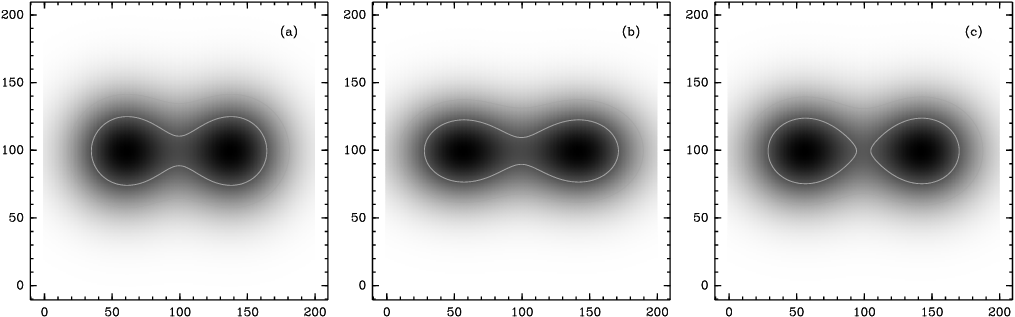
\includegraphics[width=\textwidth]{figures/toy.png}

  \caption{ Toy example of shear-dependent object detection in the presence of
    a PSF.  In panel (a) two objects are present, convolved by a PSF with no
    shear.  Contours represent constant brightness.  In panel (b) the objects
    are sheared by $\gamma = (0.0, 0.1)$ {\em after} the PSF convolution.
    Contours are the same as panel (a).  In this case the inner contours for
    the two objects overlap before and after application of the shear.  This is
    a general property of the shear transformation in the weak regime. In panel
    (c) the shear is applied {\em before} the PSF convolution, which mimics
    real sky images. In this case the inner contours do not overlap after
    shearing, and two objects may be detected rather than one.  For case (c) an
    object detection algorithm that identified connected regions above a
    threshold as a single object would manifest a shear-dependent object
    detection bias.  \label{fig:toy} }

\end{figure*}

Common object detection schemes in use today, such at those in Source Extractor
\citep{Bertin96} and the HST/LSST pipelines \citep{BoschHSC2018,BoschLSST2018}
are based on thresholding, similar to the simple approach described above but
differing in complexity and efficiency. Thus we would expect object detections
produced by those codes to also manifest shear dependence. An open question,
which we will not address in this work, is whether or not one can derive an
object detection algorithm which is independent of the shear applied to the
image in the presence of a PSF and a detector with finite spatial resolution.
Such an algorithm would in principle eliminate the shear-dependent object
detection biases explored in this work.

Current implementations of \mcal\
\citep[e.g.,][]{HuffMcal2017,SheldonMcal2017}, when used with the common object
detection schemes discussed above, are expected to exhibit shear-dependent
object detection biases. These implementations of \mcal\ work by applying
artificial shears to small postage stamp images for objects found during an
{\em independent} object detection step, run before the application of \mcal,
followed by a calculation of the response of an ellipticity measurement to the
applied shear. This independent object detection will already manifest a
shear-dependent object detection bias, and thus any shear applied when running
\mcal\ does not properly measure the full response to shear.

This shear-dependent object detection bias is a type of selection effect.
Corrections for selection effects for a static catalog were already derived in
\cite{SheldonMcal2017}, but that formalism implicitly assumes that the base
catalog itself is unaffected by selection effects.  Similarly, that formalism
cannot work near the object detection threshold, even for isolated objects,
because the object detections needed for the corrections will, by definition,
not be present in the catalog.

As we will demonstrate, object detection effects can be incorporated naturally
by shearing larger images, rather than small postage stamps, and re-running the
object detection algorithm on each of the sheared images. In this process,
shear measurement errors, selection effects, object detection, and any possible
blending effects are all accounted for.  We call this technique \mdet.

In this work, we focus on elucidating the source of shear-dependent object
detection biases and the performance of the core \mdet\ algorithm. We
demonstrate that the largest biases occur for pairs of galaxies separated by a
distance such that their images strongly overlap and one, rather than two
objects is detected in half of the cases.  Further, we provide evidence that
object deblending techniques that are based on objects detected in the image
cannot correct for the biases. Next, we demonstrate that \mdet\ can produce
unbiased shear estimates in simulations with realistic, LSST-like
\citep[e.g.,][]{chang2013} levels of object blending.  After that, we estimate
the impact of the main physical assumption made by \mdet, namely that all
objects in a small region of the sky experience the same shear. Finally, we
begin to address some of the technical challenges of implementing \mdet\ on
real imaging data by demonstrating that the technique, when applied to
multi-epoch imaging surveys, can naturally average out enough of the potential
biases associated with spatial point-spread function (PSF) variation.

The paper is laid out as follows. In Section~\ref{sec:sims}, we describe our
simulation and analysis techniques. In Section~\ref{sec:detbiases}, we study
the effects of object detection on shear measurements with \mcal.
In Section~\ref{sec:mitigate}, we describe \mdet\ which combines \mcal\ with
an object detection algorithm in order to mitigate the shear biases from object
detection. We also discuss the physical limits of \mdet\ here.
In Section~\ref{sec:psfvar}, we study the effects of the PSF variation on \mdet.
Finally, we conclude in Section~\ref{sec:conc}.

\section{Analysis and Simulation Techniques}
\label{sec:sims}

In this section, we describe our object simulation and measurement techniques.
In all cases, we use the \galsim\ \citep{GALSIM2015} software package to
generate images, perform convolutions etc. We use the \texttt{SEP} \citep{sep}
Python wrapper of the Source Extractor software package \citep{Bertin96} for
source detection as needed. Finally, we make extensive use of \ngmix
\footnote{\url{https://github.com/esheldon/ngmix/}} for object measurement and
the \mcal\ implementation.

\subsection{\textsc{Metacalibration}}

\mcal\ is a general technique that computes the linear response of image
measurements to an applied shear using only the observed image. Up to linear
order, we can write the response of an image measurement to an applied shear as

\begin{eqnarray}
\boldsymbol{e} & \approx & \left.\boldsymbol{e}\right|_{\gamma=0} +
                           \left.\frac{\partial \boldsymbol{e}}{\partial\boldsymbol\gamma}\right|_{\gamma=0} \boldsymbol\gamma +
                           O(\boldsymbol\gamma^2)\nonumber\\
               & \equiv  & \left.\boldsymbol{e}\right|_{\gamma=0} +
                           \boldsymbol{R} \boldsymbol\gamma +
                           O(\boldsymbol\gamma^2)
\end{eqnarray}
where $\boldsymbol{e}$ is the image measurement (e.g., an ellipticity
measurement), $\boldsymbol\gamma$ is the applied shear, and $\boldsymbol{R}$ is
the response (matrix) of the image measurement at zero applied shear,
$R_{ij}=\partial e_i /\partial \gamma_j$.

\mcal\ estimates this response via a numerical, finite-difference derivative
\begin{displaymath}
R_{ij} \approx \frac{e_i^{+} - e_i^{-}}{\Delta\gamma_j}\ .
\end{displaymath}
where $R_{ij}$ is the estimated response of the object to shear
and $\Delta\gamma_j = 2 \gamma_j$ is the difference between two applied
shears, $\pm \gamma_j$, with $\gamma_j$ a small shear, usually of order 0.01. The quantity
$e_i^{+/-}$ is the $i$-th ellipticity component measured on an image sheared with
$\pm\Delta\gamma_j$. In detail, one must appropriately handle the PSF and
other observational effects when computing $R_{ij}$. Note that as the
estimated responses per-object are quite noisy, they must be averaged
over many images/objects in order to estimate the response of a set of
images/objects to a shear.

In the notation above, we have denoted the object ellipticity measurement as
$\boldsymbol{e}$, but implicit is the fact that the objects must have been
detected.  We will expand on this notation to explicitly include object
detection in section \ref{sec:mitigate}.

We will focus on detection biases in this work, but there are a number of steps
in the image processing that are shear dependent: detection, centroiding,
ellipticity measurement, flux measurement, etc.  In this sense, the \mdet\
method will measure the response of all image manipulations and measurements to
an applied, constant shear.

\subsection{Multi-object Fitting Deblending}

Multi-object Fitting (MOF) deblending is a technique employed by the Dark
Energy Survey to account for blending of objects when performing image
measurements \citep{DESY1cat}. It is representative of a set of techniques that
rely on fitting models to images for a list of preexisting detections. The
model fit is then used directly to form a flux measurement or indirectly by
using it to approximately remove the light of the neighboring objects in the
image before further processing.

In this work, we use an \ngmix\ based MOF
algorithm\footnote{\url{https://github.com/esheldon/mof/}}. It is an improved
version of the MOF fitter from the DES Y1 analysis which is both more stable
and faster. It uses a linear combination of a De Vaucouleurs'
\citep{devauc1948} profile and exponential profile. The profiles are
constrained to be cocentric, coelliptical, and to have a fixed one-to-one size
ratio.  The relative amplitude of the two profiles, the fraction of the total
flux in the De Vaucouleurs' profile, is a free parameter and is allowed to vary
outside of the range [0, 1]. Finally, to process a large number of objects, we
follow \citet{DESY1cat} and break them up into interacting groups.  These
groups of objects are then simultaneously fit using a least-squares loss
function.

\subsection{Galaxy Pair Simulations}
\label{sec:sims:pairs}

In order to isolate the effects of detection easily, we first employ a
simulation setup consisting of two simulated galaxies with a variable
separation between them. By varying the separation of the objects, we can
carefully tune the effects of blending.

The galaxies are each a combination of a bulge component, modeled as a De
Vaucouleurs' profile \citep{devauc1948} and disk component modeled as an
exponential. The fraction of light in the bulge was random and ranged uniformly
between 0.0 and 1.0. The disk ellipticity was drawn from the distribution
presented in \cite{ba14}, equation 24, with ellipticity variance set to 0.20,
with a random orientation. The bulge was given the same orientation as the disk
but with ellipticity set to the disk ellipticity times a random number drawn
uniformly between 0.0 and 0.5. The half-light radius of the disk
$r_{50}^{\mathrm{disk}}$ was set to a uniform random draw between 0.4 and 0.6
arcsec. The half-light radius of the bulge was a random draw between $0.4
r_{50}^{\mathrm{disk}}$ and $0.6 r_{50}^{\mathrm{disk}}$. The bulge was shifted
from the center of the disk within a radius 0.05$r_{50}^{\mathrm{disk}}$ and in
a random direction. The light of the disk was divided between a smooth component
and a set of simulated ``knots of star formation'', represented by point sources
placed randomly with the same exponential distribution as the disk.  Between 1
and 50 knots were placed, such that the fraction light in the knots ranged
between 0.4\% and 20\%. Finally, the total flux and noise were set such that the
signal-to-noise ratio ranged uniformly between 25 and 35.

We placed two of these randomly generated galaxies in an image, with separation
ranging from 1.0 and 4.0 arcsec. The pair was placed such that the line
between the pair had a uniform random orientation relative to the coordinate
axes. Each object was given an additional random dither within a pixel. The
galaxies were treated as transparent, such that the value in a pixel was equal
to the total sum from both galaxies plus noise. The pixel scale was set to 0.263
arcseconds, appropriate for a ground-based, DES-like survey. Example images are
shown in figure \ref{fig:pairs}

\begin{figure*}
    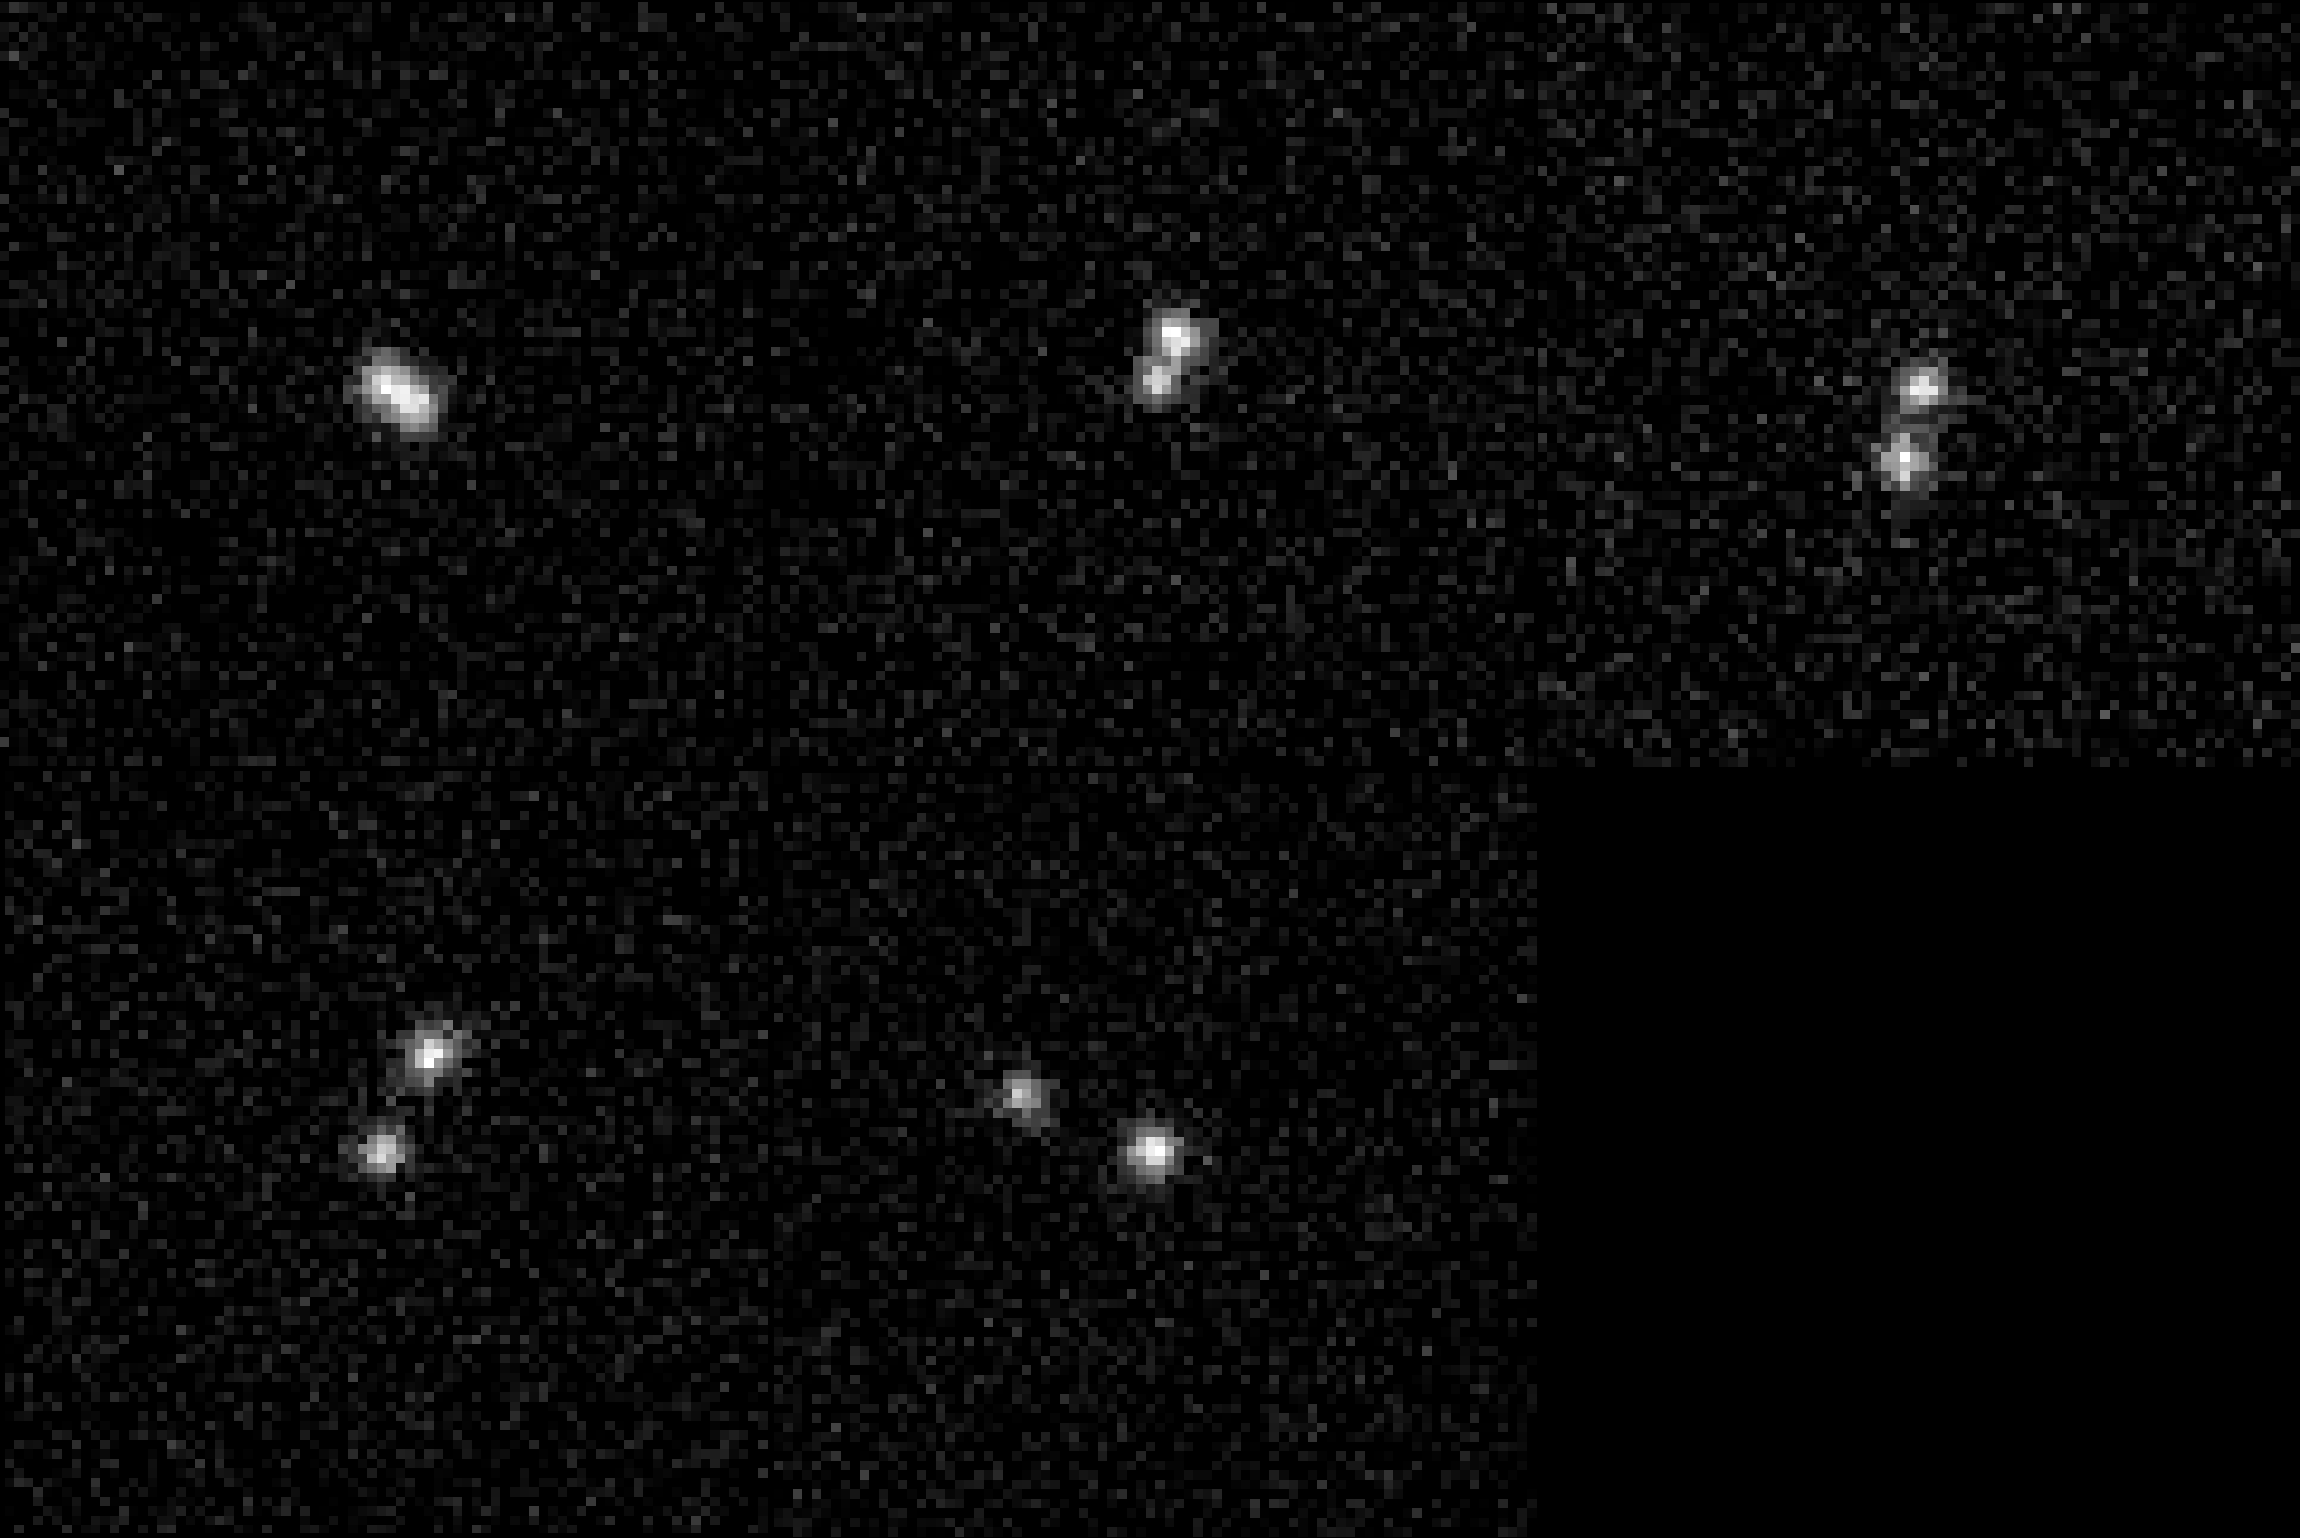
\includegraphics[width=\textwidth]{figures/bdk-comb.png}
    \caption{Example images of simulated galaxies used for the pair tests
    presented in section \ref{sec:sims:pairs}.  From left to right in the top row,
    the separations are 1.0, 1.5, 2.0 arcsec. From left to right in the bottom row the
    separations are 3.0 and 4.0 arscec. The pixel scale is 0.263 arcsec.
    \label{fig:pairs}}
\end{figure*}

\subsection{Simulations with Representative Galaxy Density and Noise}
\label{sec:sims:realgals}

We used the
\texttt{WeakLensingDeblending}\footnote{\url{https://github.com/LSSTDESC/WeakLensingDeblending}}
package to generate image simulations with realistic galaxy densities and
pixel noise for both the DES and LSST surveys. We generated images in the r-,
i-, and z-bands with an effective depth that is roughly equivalent to full 5
and 10 year coadd image for the DES and LSST respectively. For our primary
tests, we neglected the effects of PSF variation and used a constant PSF
per-band with the typical (expected) seeing for each survey ($\sim\!1$ arcsec
and $\sim\!0.8$ arcsec resepctively). We tested variable PSFs separately, as
discussed in \S \ref{sec:psfvar}.  For the DES image simulations, we have fixed
the exposure times for a single-epoch image to 90 seconds, so that the
full-depth coadd images from 10 epochs have exposure times of 900 seconds in each
filter. The depths of the LSST images
are set to match those assumed by the \texttt{WeakLensingDeblending} package for the 10 year
survey. Example images for each survey are shown in Figure~\ref{fig:simimages}.

\begin{figure*}
    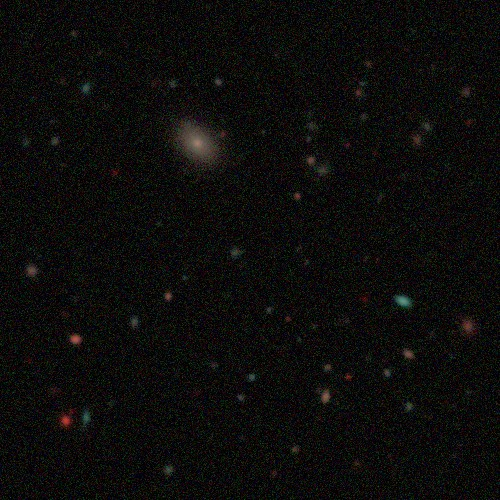
\includegraphics[width=0.9\columnwidth]{figures/des_gri.jpg}
    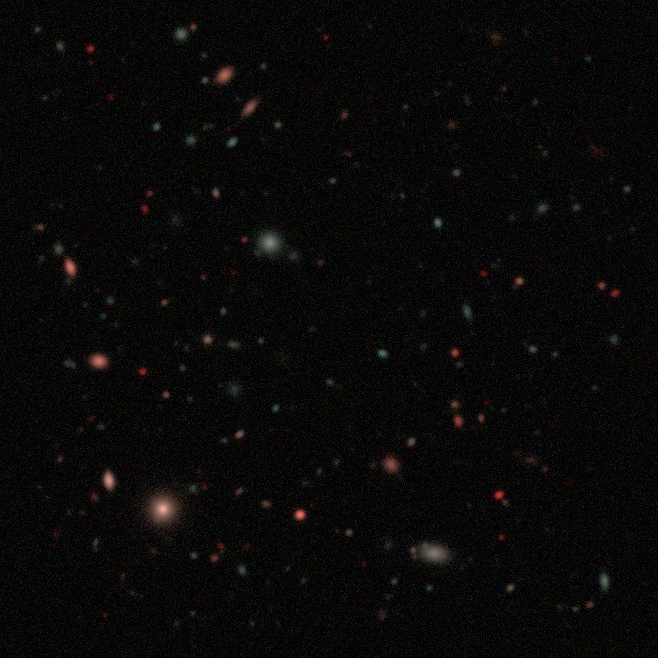
\includegraphics[width=0.9\columnwidth]{figures/lsst_gri.jpg}
    \caption{
        Example images from the DES (left) and LSST (right) simulations. Each
        multicolor, $gri$-band image is approximately $\sim\!2.2$ arcmin on a side. The
        DES images have a pixel scale 0.263 arcsec and a PSF FWHM of $\sim\!1$ arcsec.
        The LSST images have a pixel scale of 0.2 arcsec and a PSF FWHM of $\sim\!0.8$
        arcsec.
        \label{fig:simimages}}
\end{figure*}


\section{Shear-dependent Detection Biases}\label{sec:detbiases}

In this section, we employ a variety of specialized simulation setups to
elucidate the role of detection biases in \mcal\ shear measurements. We first
examine shear measurement on pairs of galaxies at various separations. We then
look at detection biases in DES- and LSST-like simulations with realistic
galaxy densities and pixel noise. We find in all cases that object detection
imparts a non-negligible shear measurement bias. As we will show in \S
\ref{sec:mdetpairs}, we can correct this bias by including detection in the
\mcal\ process, even if no explicit deblending (division of light between
objects) is performed.

\subsection{Bias in Simulations of Galaxy Pairs}

We tested \mcal\ with MOF deblending using the galaxy pair simulation presented
in \S \ref{sec:sims:pairs}. Detection was performed using \sx, with settings
matching those used for DES year 5 survey reductions (DES Collaboration, in prep.).
We got similar results using a simple local peak finder for detection.
We saw similar levels of bias with and without performing deblending using MOF.

The multiplicative bias $m$ is shown in figure \ref{fig:pairbias} as a function
of the pair distance. For a large separation of 4 arcsec, two objects are
detected in essentially all cases and no significant bias is seen.  For smaller
separations, the two objects overlap more significantly and the detection
becomes more ambiguous, with only one object detected in some cases.  The bias
grows as the separation decreases, with the maximum bias occurring at about 1.5
arcsec separation. At 1.5 arcsec separation the detection is most ambiguous,
with two objects detected in half the cases. For smaller separations the
objects overlap more and detection becomes less ambiguous, with one object
detected in more than half of the cases. At separations of 1 arcsec, the two
objects are detected as one essentially in every case, and again no significant
bias is detected.

\begin{figure}
    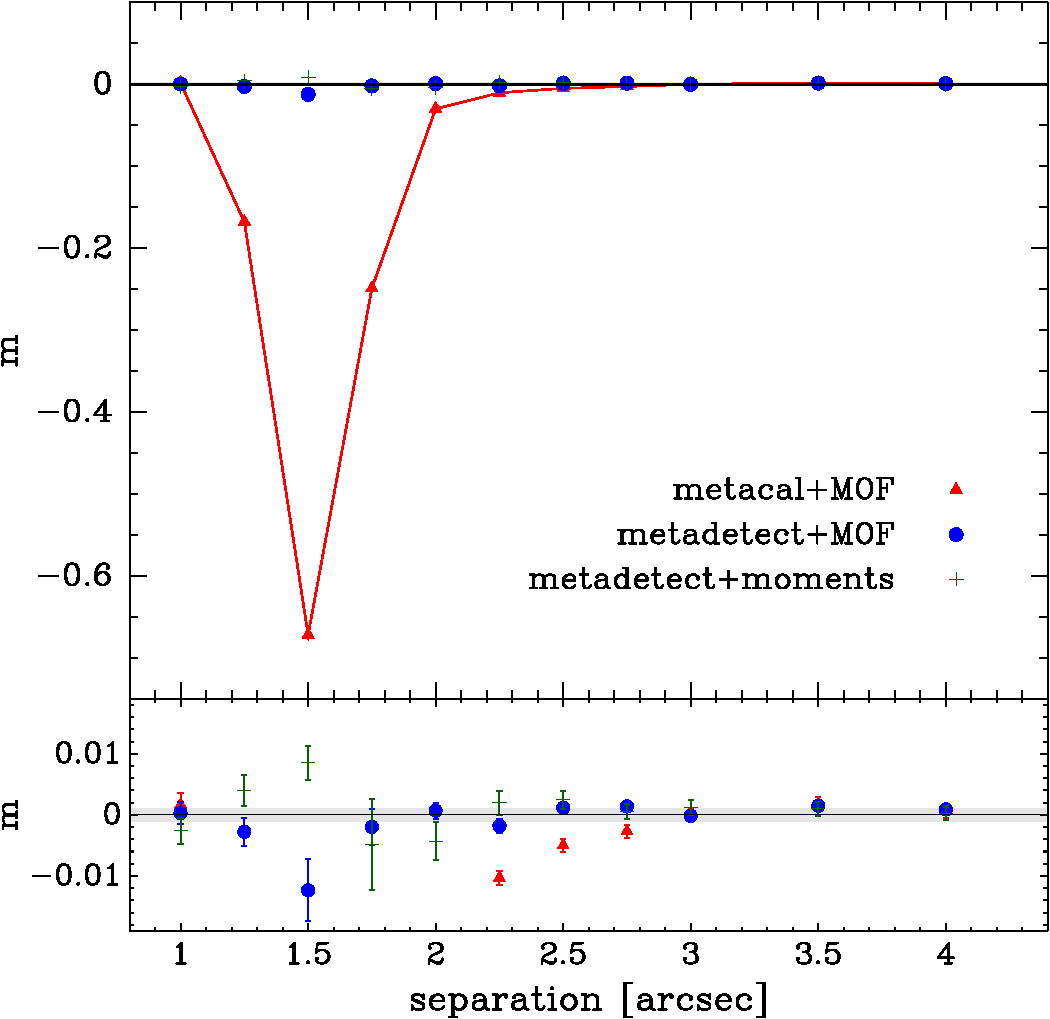
\includegraphics[width=\columnwidth]{figures/pairs-mc-bdkpair.pdf}

    \caption{Mean multiplicative shear bias measured for pairs of simulated
    galaxies (see \S \ref {sec:sims:pairs} for details) at various separations.  At
    each separation, a large number of trials was generated with random
    orientations of the pair.  At 4.0 arcsec separation, two objects were
    detected in all cases.  At 1.5 arcseconds two objects were detected in half
    the cases.  At 1.0 arcsec a single object was detected in all cases.  Red
    triangles represent standard \mcal\ with MOF deblending for modeling all
    detected objects.  Blue circles represent \mcal+MOF with detection included
    as part of the process.  Green pluses represent \mcal\ with detection
    included but without deblending, and using simple weighted moments without
    PSF correction as the shear estimator. Very large biases are seen for
    standard \mcal+MOF as detection becomes ambiguous, for example at 1.5
    arcsec separations.  When detection is included in the \mcal\ process the
    biases are greatly reduced.  The bias is reduced even in the case where no
    deblending was performed and no PSF correction or detailed object modeling
    were performed.  This indicates the large majority bias is due to
    shear-dependent detection, not light blending or details of the object
    modeling.
    \label{fig:pairbias}}

\end{figure}

The correspondence between detection ambiguity and shear bias is a hint that
the bias is caused by shear-dependent detection. Next, we perform simulations
of DES- and LSST-like surveys and show explicitly that by turning object
detection off, we can eliminate these detection biases.

% raw outputs
% DES mcal+MOF
% s2n: 10
%     # of sims: 49499
%     m       : -0.066781 +/- 0.009613
%     c       : -0.000055 +/- 0.000371
% s2n: 15
%     # of sims: 49496
%     m       : -0.050463 +/- 0.008567
%     c       : 0.000271 +/- 0.000416
% s2n: 20
%     # of sims: 49476
%     m       : -0.037302 +/- 0.007727
%     c       : 0.000201 +/- 0.000449

% LSST mcal+MOF
% s2n: 10
%     # of sims: 49014
%     m       : -0.082423 +/- 0.005180
%     c       : -0.000245 +/- 0.000192
% s2n: 15
%     # of sims: 49014
%     m       : -0.066753 +/- 0.004539
%     c       : -0.000173 +/- 0.000197
% s2n: 20
%     # of sims: 49014
%     m       : -0.062331 +/- 0.004279
%     c       : -0.000094 +/- 0.000210

% DES shear scene
% s2n: 10
%     # of sims: 9997419
%     m       : 0.000161 +/- 0.000857
%     c       : -0.000011 +/- 0.000034
% s2n: 15
%     # of sims: 9982020
%     m       : 0.000407 +/- 0.000786
%     c       : -0.000036 +/- 0.000039
% s2n: 20
%     # of sims: 9928501
%     m       : 0.000814 +/- 0.000754
%     c       : -0.000013 +/- 0.000044

% LSST shear scene
% s2n: 10
%     # of sims: 9996600
%     m       : 0.000472 +/- 0.000433
%     c       : -0.000024 +/- 0.000018
% s2n: 15
%     # of sims: 9996600
%     m       : -0.000015 +/- 0.000339
%     c       : -0.000003 +/- 0.000017
% s2n: 20
%     # of sims: 9996600
%     m       : 0.000190 +/- 0.000284
%     c       : -0.000012 +/- 0.000018

% DES no shear scene
% s2n: 10
%     # of sims: 9995117
%     m       : -0.003574 +/- 0.001228
%     c       : -0.000043 +/- 0.000037
% s2n: 15
%     # of sims: 9983339
%     m       : -0.000999 +/- 0.000997
%     c       : -0.000057 +/- 0.000040
% s2n: 20
%     # of sims: 9938170
%     m       : -0.002601 +/- 0.000948
%     c       : -0.000017 +/- 0.000044

% LSST no shear scene
% s2n: 10
%     # of sims: 9999000
%     m       : -0.004659 +/- 0.000559
%     c       : -0.000024 +/- 0.000018
% s2n: 15
%     # of sims: 9999000
%     m       : -0.003514 +/- 0.000430
%     c       : -0.000003 +/- 0.000018
% s2n: 20
%     # of sims: 9999000
%     m       : -0.002873 +/- 0.000367
%     c       : -0.000022 +/- 0.000019


\begin{table*}
  \centering
  \caption{
    Multiplicative biases in weak lensing simulations for various shear
    measurement techniques. In all cases, the simulations use realistic
    galaxy ellipticities, galaxy sizes and noise for the given survey. For measurements using standard \mcal\ with
    MOF deblending, a cut of $T/T_{PSF} > 0.5$ was also applied. Measurements with
    \mdet\ and moments used a size cut of $T/T_{PSF} > 1.2$. In the case of \mdet\ with moments,
    no deblending corrections are applied and the moments are a simple weighted moment
    with no PSF correction.}
  \label{tab:shearmeas}

  \begin{tabular}{|l|l|l|c|c|}
    \hline
    Simulation & Method & Full Scene Sheared? & \snr\ Cut & m \\
    \hline

    \hline
    \multicolumn{5}{c}{metacal+MOF - full scene sheared}\\
    \hline
    DES   & metacal+MOF & yes & \snr$ > 10$ & $-0.067 \pm 0.010$  \\
    DES   & metacal+MOF & yes & \snr$ > 15$ & $-0.050 \pm 0.009$  \\
    DES   & metacal+MOF & yes & \snr$ > 20$ & $-0.037 \pm 0.008$  \\
    \hline
    LSST  & metacal+MOF & yes & \snr$ > 10$ & $-0.082 \pm 0.005$  \\
    LSST  & metacal+MOF & yes & \snr$ > 15$ & $-0.067 \pm 0.005$  \\
    LSST  & metacal+MOF & yes & \snr$ > 20$ & $-0.062 \pm 0.004$  \\
    \hline

    \hline
    \multicolumn{5}{c}{metadetect+moments - full scene sheared}\\
    \hline
    DES   & metadetect+moments & yes & \snr$ > 10$ & $+0.00016 \pm 0.00086$  \\
    DES   & metadetect+moments & yes & \snr$ > 15$ & $+0.00041 \pm 0.00079$  \\
    DES   & metadetect+moments & yes & \snr$ > 20$ & $+0.00081 \pm 0.00075$  \\
    \hline
    LSST  & metadetect+moments & yes & \snr$ > 10$ & $+0.00047 \pm 0.00043$  \\
    LSST  & metadetect+moments & yes & \snr$ > 15$ & $-0.00002 \pm 0.00034$  \\
    LSST  & metadetect+moments & yes & \snr$ > 20$ & $+0.00019 \pm 0.00028$  \\
    \hline

    \hline
    \multicolumn{5}{c}{metadetect+moments - individual objects sheared}\\
    \hline
    DES   & metadetect+moments & no & \snr$ > 10$ & $-0.0036 \pm 0.0012$  \\
    DES   & metadetect+moments & no & \snr$ > 15$ & $-0.0010 \pm 0.0010$  \\
    DES   & metadetect+moments & no & \snr$ > 20$ & $-0.0026 \pm 0.0009$  \\
    \hline
    LSST  & metadetect+moments & no & \snr$ > 10$ & $-0.0047 \pm 0.0006$  \\
    LSST  & metadetect+moments & no & \snr$ > 15$ & $-0.0035 \pm 0.0004$  \\
    LSST  & metadetect+moments & no & \snr$ > 20$ & $-0.0029 \pm 0.0004$  \\
    \hline
  \end{tabular}

\end{table*}

\subsection{Bias in Simulations with Representative Galaxy Density and Noise}

We now explore the effects of detection in simulations that are representative
of real survey images. As a baseline, we note that \mcal\ with MOF deblending
and \sx\ detections results in catastrophic biases, $\sim-5\%$, for a DES-like
survey. Simulations of LSST-like surveys demonstrate even larger biases.See
Table~\ref{tab:shearmeas} for details. Note also that this procedure closely
matches that currently done with DES data.  We see similar biases when no
de-blending is performed.   

In order to unpack the source of the bias in this case, we compare two
different \mcal\ shear measurements. The first \mcal\ shear measurement is done
on a catalog of the true source positions using a fixed 1.2 arcsecond Gaussian
weighted moment ellipticity measurement. The second employs \mcal\ with the
same ellipticity measurement, but using \sx\ detections instead of the true
object positions. We find that while the first \mcal\ shear measurement is
unbiased ($-0.0011\pm0.0012$), the second exhibits a bias of
$-0.058\pm0.001$.\footnote{The simulations with the true source positions are
computationally slow because they involve measurements on all sources, even
ones which are undetectable. Thus we were unable to decrease the errors on the
multiplicative bias below $\sim0.1\%$. However, for simulations with round,
exponential, high signal-to-noise objects only, we have found that \mcal\ with
the true source positions and a weighted moment has bias ($0.00033 +/-
0.00009$) in the presence of blending, consistent with the bias expected due to
the breakdown of the weak lensing approximation.} Note that this ellipticity
measurement makes no corrections for object blending, but in the case where we
use the true object positions, it is still unbiased. Thus we have demonstrated
that given a set of true source locations, \mcal\ is not sensitive to
blending.\footnote{In practice, we have found that when using \mcal\ with true
detections and more complicated ellipticity measurements, for example using a
non-linear model fit, biases can reappear. Thus whether or not a \mcal\
ellipticity measurement is biased due to blending depends sensitively on the
technique used to measure ellipticities on the sheared \mcal\ images.}

This set of tests also demonstrates explicitly that source detection can cause
significant shear measurement biases even for techniques which are robust to
blending. The source detection biases probably originate from multiple causes.
One of those causes is undoubtedly related to merging or splitting objects in a
way which depends on the underlying shear, as illustrated with a toy example in
Figure~\ref{fig:toy} and the galaxy pair tests above.

\begin{comment}
We have found that even for extremely high signal-to-noise exponential objects
placed on a grid, using \mcal\ with the Gaussian weighted moments around object
centers determined by \sx\ still results in small biases, $\sim\!-0.2\%$. Thus
at least some of the biases have to do with the effect of the underlying shear
on object centering:  as demonstrated in \cite{SheldonMcal2017}, this
centroiding bias is corrected as part of the ordinary \mcal\ shear response
when center is re-fit on sheared images and detection is unambiguous, but no
such re-determination of the position was allowed in this case.  As we will
demonstrate below, once we include object detection in the \mcal\ process, we
can simultaneously correct for such measurement effects and shear-dependent
detection effects.
\end{comment}


\section{Mitigating Shear-dependent Detection Biases with \textsc{METACALIBRATION}}
\label{sec:mitigate}

In the previous section, we demonstrated that source detection is a significant
source of bias in shear measurements with \mcal. Here we test a
straight-forward fix for this bias, namely including source detection in the
\mcal\ process. We have implemented this fix as follows. We take relatively
large images (typically $\sim$ 2 arcminute on a side) and apply \mcal\ directly
to the full image using the PSF at the center of the image for deconvolutions.
For each of the five \mcal\ images, we apply \sx\ to detect sources. We then
measure shears in postage stamps around each detection in each image using an
non-PSF corrected, Gaussian-weighted moment.  These five catalogs are then
combined into a single estimate for the shear in the patch by computing the
average shear response for the image
\begin{eqnarray}
\langle \boldsymbol\gamma \rangle &\approx& \langle \boldsymbol{R}\rangle^{-1}\langle\boldsymbol{e}\rangle\\
\langle R_{ij}\rangle &=& \frac{\langle e_i^{+}\rangle - \langle e_i^{-}\rangle}{\Delta\gamma_j}
\end{eqnarray}
where the equation for the response above is for a single shear component. We term this
process \mdet.

Note that the averages above are over the {\it catalogs} from running source
detection and ellipticity measurement on differently sheared images. This is in
effect the ``total derivative'' response, shown in section 3 of
\cite{SheldonMcal2017}, without any attempt to split the response into the
shear response and selection response using the chain rule.  Individual shear
responses, as used in both \cite{SheldonMcal2017} and \cite{HuffMcal2017}, are
not calculated.  Doing so would require matching the lists of detections found
on the different sheared images, so that finite differences for each object
could be formed.  This act of matching would introduce the very shear-dependent
object detection biases we wish to calibrate.  We will discuss the implications
of this fact the analysis of imaging surveys in \S \ref{sec:wavg}.

\subsection{Results for Simulated Galaxy Pairs}
\label{sec:mdetpairs}

In figure \ref{fig:pairbias} we show results for the pairs of galaxies, including
detection in the \mcal\ process. The blue filled circles represent the case
where deblending is performed using MOF. The green plus signs represent the
case where no deblending was performed. For the undeblended case we further
simplified the process: simple weighted moments were taken at the position
determined by \sx\ using a fixed weight function with full-width at half
maximum 1.2 arcsec, without any correction for the PSF.

In both cases the bias is greatly reduced, with significant bias seen only at
the special separation of 1.5 arcsec, where the two objects are detected as one
object in half of the cases. This demonstrates that the bias we see is not
primarily due to the process of deblending itself, but rather shear-dependent
detection effects. The remaining biases at 1.5 arcsec tend to be different sign
for the deblended and non-deblended cases, which shows there is a qualitative
difference in how the two measurements respond to the shear. As we will show
below, we find no significant net bias for more realistic DES and LSST-like
images where the typical separation of galaxies is not at a special location of
maximum detection ambiguity.

\subsection{Results for Simulations with Representative Galaxy Density and Noise}
\label{sec:res:constpsf}

We show results for DES-like and LSST-like surveys in Table~\ref{tab:shearmeas}.
We have used a constant PSF and constant shear for these simulations. We find
that in all cases our \mdet\ shear measurements are unbiased up to
second-order shear effects. This conclusion holds despite the extensive blending
of the object images and the large source detection effects we documented
above. They also meet or exceed the requirements for analyzing an LSST-like survey
\citep[e.g.,][]{huterer2006}.

\subsubsection{Testing the Physical Assumptions Behind \mdet}

Here we address a key physical assumption made by \mdet, namely that the full
scene is transformed by a constant shear. In such an image, the space between
objects is sheared in the same way the objects are. This shearing of the full
scene matches the \mdet\ shearing steps exactly and thus allows us to calibrate
the mean shear in the image to high precision. A realistic image with a mix of
objects under different shears at different redshifts can be thought of as a
sum of a series of constant shear images with the full scene sheared
independently for each image in the sum.  This image would not exactly match
the \mdet\ process and thus we might expect some residual bias in the shear
calibration.  Note that non-constant shear, in the sense that objects from
widely separated parts of the sky will have different shears, is not in itself
a source of bias, because it is the mean shear or other statistic that is
recovered by the formalism \citep{SheldonMcal2017}.

In order to obtain an estimate and bound on this effect, we make a simple
modification to our simulations. When building them, rather than shearing the
full scene to impart the true shear to the image, we shear each object
individually and then add it to the image. This modification leaves the space
between objects unsheared, which is maximally different from what happens
during the \mcal\ image shearing process. Results for these simulations are in
the bottom rows of Table~\ref{tab:shearmeas}. We find small residual biases in
this case, of order $\sim-0.3\%$.

We expect these biases to depend on the density of blended objects in the
survey, with larger residual biases for LSST-like surveys than DES-like
surveys.  Understanding the expected level of this bias in real surveys will
require further study, and is beyond the scope of this work.

\section{Handling PSF Variation}
\label{sec:psfvar}

In order to apply \mdet\ to a real, multi-band, multi-epoch survey like the DES
or LSST, we will need to be able to handle realistic levels of PSF variation,
missing data, and non-trivial WCS transformations. We will address these issues
more fully in future work, currently in preparation. However, here we will
address the issue of PSF variation, which is technically the most challenging
because \mdet\ requires deconvolution by the PSF over relatively large regions
of sky. Here, we will show that the image coadding process used in a realistic
multi-epoch survey naturally reduces the PSF variation enough to render any
associated biases negligible.

For these simulations, we use a simple population of galaxies that have
exponential profiles with a half light radius of 0.5 arcsec and a PSF with a
Gaussian profile with a full-width-at-half-maximum of 0.9 arcsec. All of the
objects are round and are rendered at a signal-to-noise of over 20. These
simulations have the advantage of having very low ellipticity noise and so are
ideal for tests that need to reach high-precision quickly. We create the images
for the simulation by coadding a number of images with random, variable PSFs.
\mdet\ is then performed using the coadd of PSF models from the input images,
with the PSF from each input image generated at the location of the center of
the final coadd.  This model is correct only at that one location, so we
expect a bias in the recovered shear.

In order to place an upper bound on this effect, we have created a variable PSF
model that has significantly more variation than we expect in real data. See
Appendix~\ref{app:pspsf} for details.  Using a single PSF realization from
Appendix~\ref{app:pspsf}, without stacking, we find a multiplicative bias of
$-0.0065 +/- 0.00044$.  However, when stacking thirty of these models, which is
the expected number of epochs for three bands in the final DES data set, we
find a multiplicative bias of only $-0.00035 +/- 0.00037$.  For LSST many more
epochs will be available for coadding.   While this test is not conclusive, we
expect that in a realistic survey scenario, PSF variation will not be a
fundamental limitation for \mdet.

\section{Implications for Survey Analysis} \label{sec:wavg}

The fact that five separate catalogs must be used without any attempt at
matching them (see \S \ref{sec:mitigate}), has implications for using \mdet\ in
the analysis of surveys.  Typically a single reference or ``gold'' sample of
objects is constructed and used for all subsequent calculations, such as
finding a redshift distribution.  With \mdet, multiple such catalogs, one for
each artificial shear, must be constructed in order to understand the response
of a summary statistics to shear.

When calculating averages for related quantities, such as a redshift
distribution, the shear response provides the appropriate weight on an
object-by-object basis \citep{SheldonMcal2017}.  But individual responses
cannot be calculated with \mdet, because this would require matching the
catalogs produced from the different artifically sheared images, which would
introduce shear-dependent selection effects.  With \mdet, in order to get an
appropriate weight, the appropriate mean response can be calculated.  For
example, when constructing a redshift distribution one could define fine
redshift bins and calculate the mean response in those bins, using the separate
sheared versions of the catalogs. This mean weight as a function of redshift
could then be interpolated to provide weights for objects when constructing the
overall redshift distribution.


\section{Summary}\label{sec:conc}

In this work, we have explored how \mcal\ weak lensing measurements perform in
realistic scenarios where a large fraction of the objects overlap and the
detection of objects can be ambiguous. These conditions will characterize all
future weak lensing surveys, especially those executed beneath the atmosphere,
so accurate performance in this regime is critical to attaining maximal
scientific knowledge from the surveys. We find that \mcal\ used with MOF-like
object deblending techniques has severe, many percent biases that get worse
with the degree of object blending. We then demonstrated that by including the
detection of objects in the \mcal\ process, we can eliminate these biases at
high precision even for an LSST-like survey. This technique, which we call
\mdet, appears to be extremely promising for future surveys.

Future work will need to continue to address a number of technical challenges
associated with implementing \mdet\ on real data. Beyond PSF variaton, larger
images can have non-trivial world coordinate system (WCS) variation.  Usually
these observational details are approximately constant over small post-stamps
and so can be dealt with easily, but this may not be so for the larger regions
which will be coadded for \mdet. Larger regions of images can have non-trivial
masking patterns due to stellar diffraction spikes, cosmic rays, etc. In the
implementation presented in this work, we use fast Fourier transforms (FFTs) to
handle convolutions, which do no permit missing data, so the masked regions
must be interpolated in some way.  In order to reconstruct accurate psf models
for the coadd, the original images can have no edges within the coadd region,
necessitating some loss of precision \citep{ArmstrongCoadd}.  Finally, the five
separate \mdet\ catalogs must each be incorporated into the full set of
downstream analysis tasks (e.g., photometric redshift estimation, the
construction of summary statistics, etc.) in order to be used for cosmological
constraints. The degree to which we can handle all of these technical
challenges will ultimately determine the accuracy of \mdet\ when used to
analyze imaging survey data.

\bibliographystyle{mnras}
\bibliography{references}

\appendix

\section{Fast Approximate Variable PSF Models}\label{app:pspsf}

\begin{figure*}
  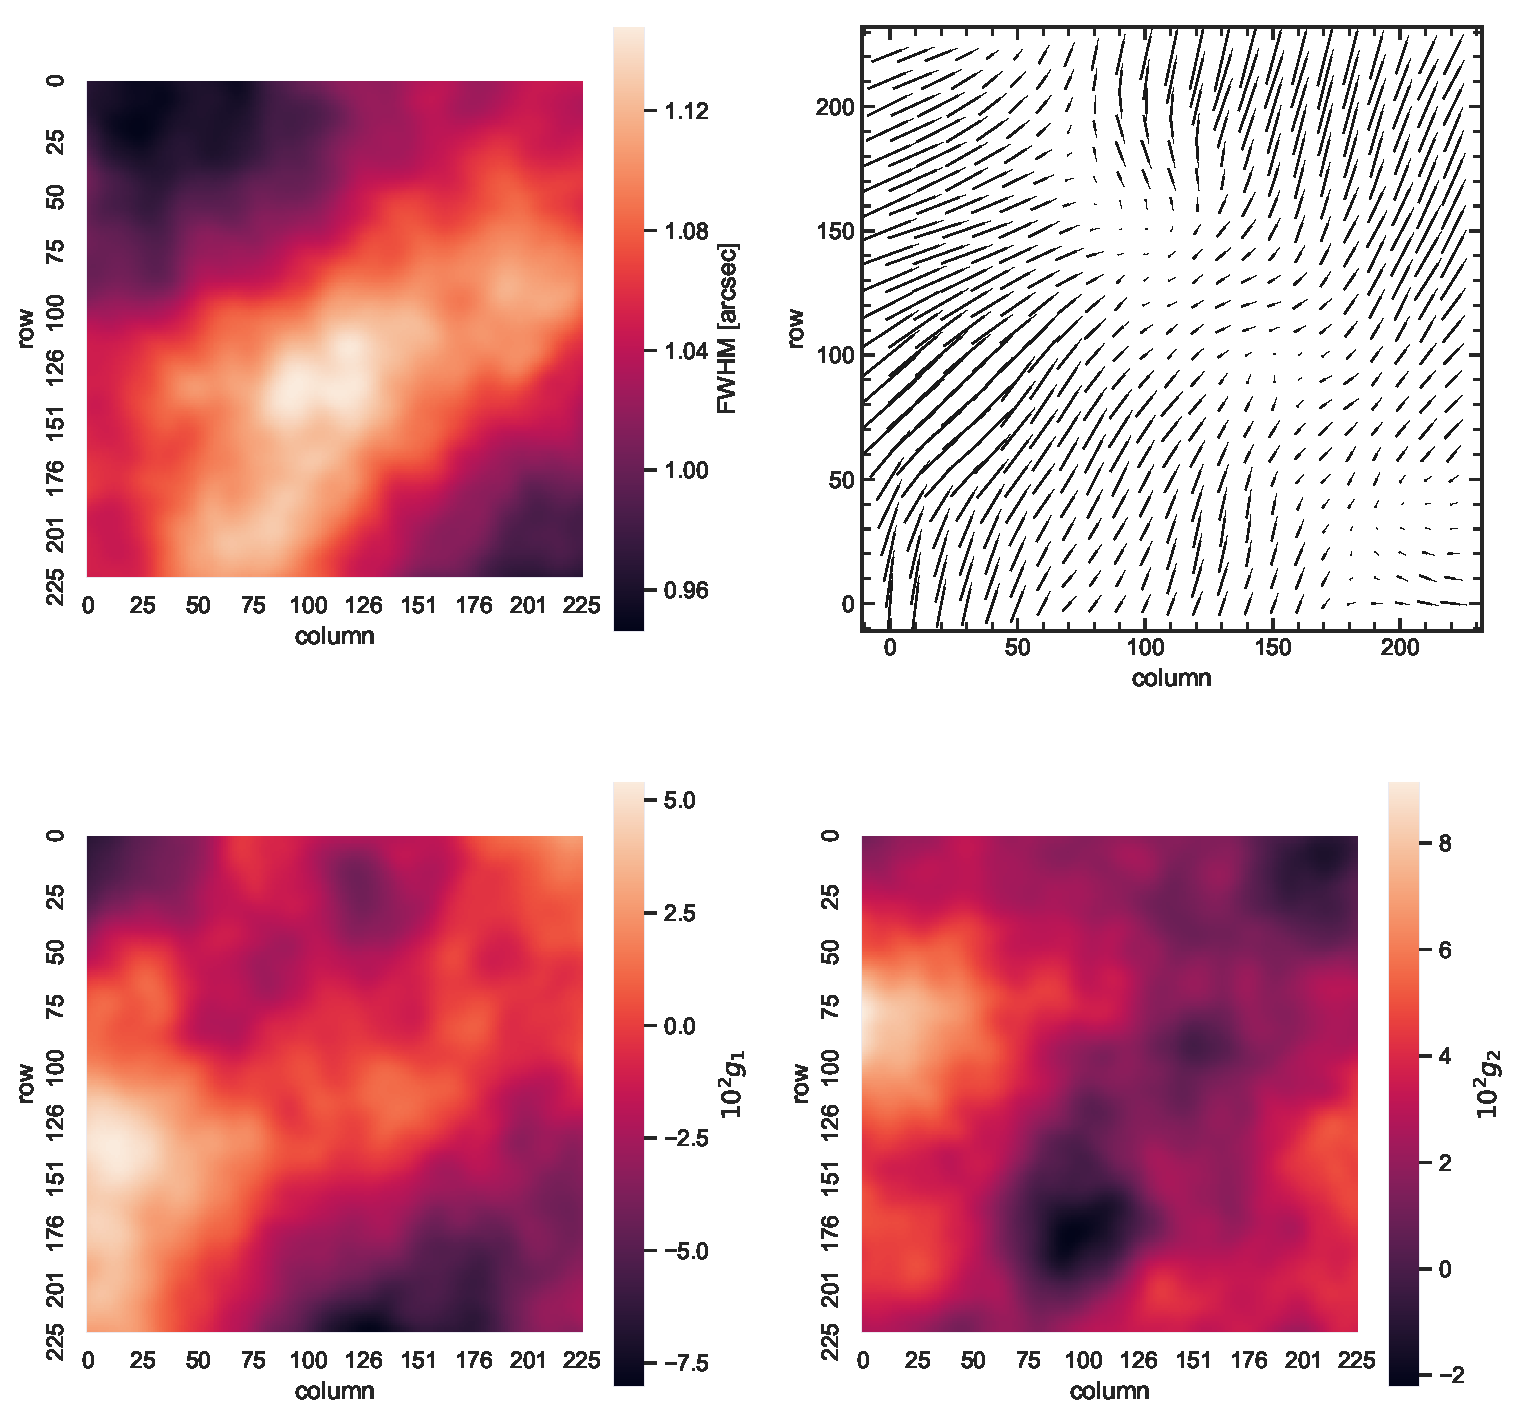
\includegraphics[width=\textwidth]{figures/pspsf.pdf}
  \caption{
    Variable PSF model statistics for a DECam-like exposure. The top-left
    panel shows the variation in the FWHM in arcseconds. The top-right panel
    shows a visualization of the PSF ellipticity variation. The bottom-left panel shows
    the variation in the $1$-component of the PSF ellipticity. The bottom-right panel
    shows the variation in the $2$-component of the PSF ellipticity. The variation in
    this model is $\gtrsim10\times$ larger than the typical PSF variation for
    either DECam or expected LSST observations. The pixel scale is 0.263 arcsec
    so that each panel is approximately 1 arcmin on a side.
    \label{fig:pspsf}}
\end{figure*}

\begin{figure}
  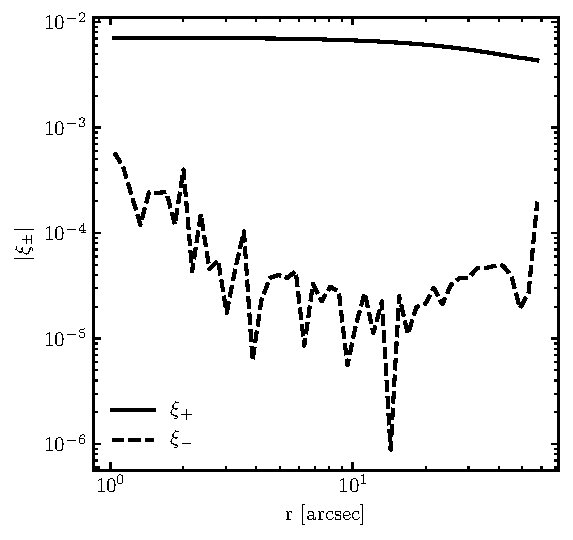
\includegraphics[width=\columnwidth]{figures/psxi.pdf}
  \caption{
    Variable PSF model shear correlation functions for a DECam-like exposure. LSST
    is expected to have shear correlation function magnitudes around
    $\sim\!10^{-4}$ \citep{jee2011}.
    \label{fig:psxi}}
\end{figure}


In this work we use a fast, approximate variable PSF model. This model eases the
computational requirements for the simulations while also retaining the
essential features of realistic PSF variation. In this appendix, we present
the model and verify its statistical properties against more realistic PSF models.

We start with the results of \citet{heymans2012}. They fit the \vonkarman model
of atmospheric turbulence

\begin{displaymath}
  P(\ell) \propto \left(\ell^{2} + \frac{1}{\theta_{0}^2}\right)^{-11/6}
\end{displaymath}
to images with high stellar density. Here $\theta_{0}$ is the outer scale of
turbulence. \citep{heymans2012} find that $\theta_{0}\approx3$ arcmin.
We further add an additional Gaussian truncation of the power

\begin{displaymath}
  P_{trunc}(\ell) \propto P(\ell)\exp\left(-\ell^2r^{2}\right)
\end{displaymath}
at a scale of $r=1$ arcsec in order to reduce the level of resulting
PSF variation. Below we show that even with this modification, our models
still have more power than a realistic model for a survey, making them useful
for providing upper limits on the effects of PSF variation.

Using this model, we seed equal amounts of E- and B-mode power on a grid of
$128\times128$ cells using random phases. Each cell of the grid is one
arcsec in size. We normalize the overall ellipticity variance to $0.10^2$. We then use
the $g1$ and $g2$ components of this model to set the variation of the ellipticity of
the PSF. We draw the mean ellipticity for each image from a Gaussian distribution of
variance $0.10^2$. Note that we also bound the total ellipticity to at most 0.5.
We model the PSF profile as a Moffat with shape parameter $\beta=2.5$.
The size of the Moffat profile is set to be proportional to $\mu^{-3/4}$,
where $\mu$ is the magnification computed from the power spectra realization. The
proportionality constant is drawn randomly from a log-normal model with
scatter 0.1 arcmin and a central value set so the final PSF size mimics a DES-like
survey.

We show an example PSF for a DES-like survey in Figure~\ref{fig:pspsf}.  Over a
1 square arcminute patch, our approximate models generate PSF ellipticity and size
variation that are $\gtrsim10\times$ that seen in real 90 second exposures
with DECam \citep{DESY1shear}, or the expected variation in a 15 second exposure with
LSST \citep{jee2011} over similar scales. Figure~\ref{fig:psxi} shows the $\xi_{\pm}$ shear correlation
functions averaged over 100 realizations of our models. For comparison, we
expect at most shear correlation function amplitudes of $\sim10^{-4}$ for LSST
\citep{jee2011} and for DESCam 90 second exposures. The DECam models were generated
using the methods of \citet{jee2011} but for DECam-like environmental conditions. For
the optical contributions to the PSF, we use a set of randomly drawn
aberrations (similar to GREAT3 \citep{great3}), but with values more typical of
DECam observations\footnote{\url{https://github.com/GalSim-developers/GalSim/blob/releases/2.1/examples/great3/cgc.yaml}}.


\bsp
\label{lastpage}
\end{document}
